% --------------------------------------------------------------------------------

\begin{exercise}

Bestimmen und skizzieren Sie diejenigen Gebiete in $R^2$, fur welche die folgenden Differentialgleichungen jeweils elliptisch, parabolisch oder hyperbolisch sind:

\begin{enumerate}[label = (\roman*)]
    \item $(y^2 + 1) u_{xx} + 2 x u_{xy} + 9 u_{yy} - u u_y = y^2 - x$,
    \item $x u_{xx} + 2 y u_{xy} + u_{yy} + x u_x = 1$.
\end{enumerate}

\end{exercise}

% --------------------------------------------------------------------------------

\begin{solution}

Wir erinnern uns an die allgemeine Form aus dem Skriptum (bzw. der Vorlesung) ...

\begin{figure}[h!]
    \centering
    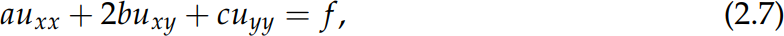
\includegraphics{../(2-7).png}
\end{figure}

... und an die Definitionen von elliptisch, parabolisch und hyperbolisch ...

\begin{figure}[h!]
    \centering
    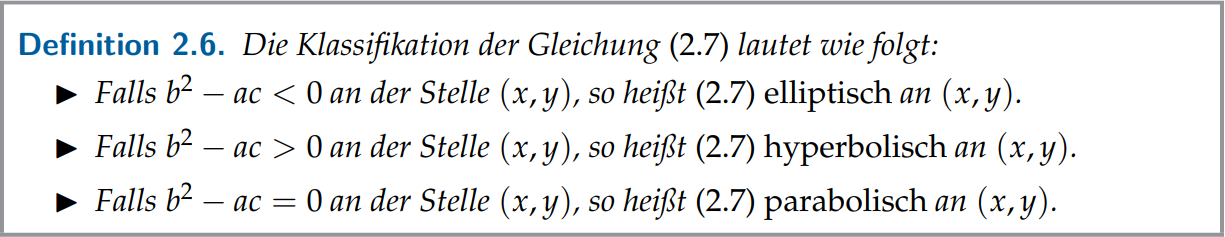
\includegraphics{../Definition 2-6.png}
\end{figure}

\begin{enumerate}[label = (\roman*)]

    \item

    \begin{align*}
        a & = y^2 + 1 \\
        b & = x \\
        c & = 9 \\
        f & = y^2 - x + u u_y
    \end{align*}

    \begin{align*}
        0 \stackrel{!}{=}
        b^2 - ac
        =
        x^2 - 9 (y^2 + 1)
        \implies
        x = \pm 3 \sqrt{y^2 + 1}
    \end{align*}

    \begin{figure}[h!]
        \centering
        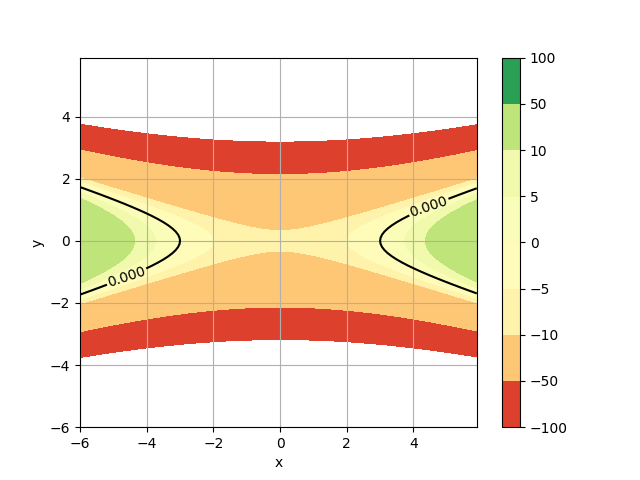
\includegraphics{../2-1-1.png}
        \caption{$x = \pm 3 \sqrt{y^2 + 1}$}
    \end{figure}

    \item

    \begin{align*}
        a & = x \\
        b & = y \\
        c & = 1 \\
        f & = 1 - x u_x
    \end{align*}

    \begin{align*}
        0 \stackrel{!}{=}
        b^2 - ac
        =
        y^2 - x
        \implies
        x = y^2
    \end{align*}

    \begin{figure}[h!]
        \centering
        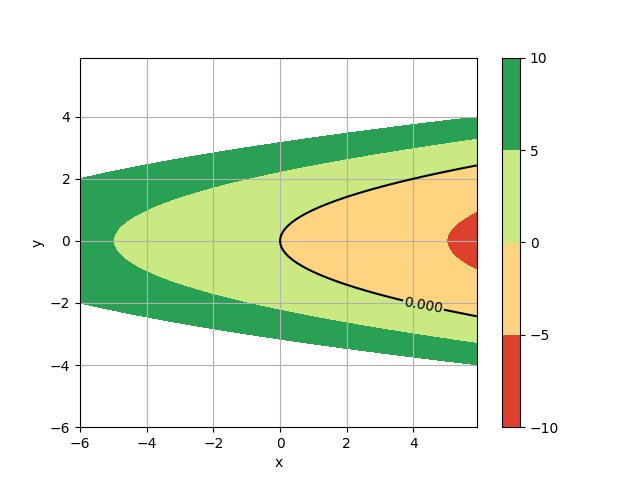
\includegraphics{../2-1-2.png}
        \caption{$x = y^2$}
    \end{figure}

\end{enumerate}

\FloatBarrier
\end{solution}

% --------------------------------------------------------------------------------
